\documentclass[a4paper, 11pt]{article}
\usepackage[T1]{fontenc}
\usepackage[utf8]{inputenc}
\usepackage{lmodern}
\usepackage{geometry}
\usepackage{url}
\usepackage{xcolor}
\usepackage{amsmath}
\usepackage{amsfonts}
\usepackage{amssymb}
\usepackage{graphicx}
\usepackage{combelow}
\usepackage[unicode]{hyperref}
\hypersetup{
  colorlinks=false,          % boxes instead of colored text
  pdfborder={0 0 1},         % box thickness (0 0 1 = thin box)
  citebordercolor=green,     % green boxes for citations
  linkbordercolor=red,       % boxes for \ref, \eqref, etc.
  urlbordercolor=blue
}
\usepackage{float}
\usepackage{indentfirst}
\usepackage{booktabs}
\usepackage{array}
\usepackage{cite}
\usepackage{caption}
\usepackage{subcaption}
\usepackage{multirow}
\usepackage{algorithm}
\usepackage{algpseudocode}
\usepackage{tikz}
\usepackage{listings}

\usetikzlibrary{arrows.meta, positioning}

\algrenewcommand\algorithmicrequire{\textbf{Input:}}
\algrenewcommand\algorithmicensure{\textbf{Output:}}

% Terraform / HCL snippets
\lstdefinestyle{hcl}{
    basicstyle=\ttfamily\footnotesize,
    keywordstyle=\color{blue!70!black}\bfseries,
    morekeywords={resource, variable, module, output, locals, data},
    morecomment=[l]{\#},
    commentstyle=\color{gray},
    showstringspaces=false,
    breaklines=true,
    frame=single,
    framesep=4pt,
}

\newcommand{\tool}{\texttt{tfimpact}}

\linespread{1}
\geometry{a4paper,top=3cm,left=3cm,right=2.5cm,bottom=2cm}

\title{
    {\huge \textbf{Computational Intelligence in Software Engineering}} \\[1.5ex]
    {\Large \textbf{Learning Where Terraform Changes Propagate: \\ A Genetic Algorithm for IaC Block-Level Co-Change Impact}}
}

\author{\textbf{Author:} Tudor-Octavian Mih\u{a}i\c{t}\u{a}\\ \textbf{Group:} ICA 246-2}

\begin{document}

\maketitle

\begin{abstract}
\textbf{Infrastructure-as-Code (IaC)} files describe cloud infrastructure as interdependent code blocks, so
editing one block often requires changes elsewhere: a renamed variable breaks the module calls that
pass it, a removed resource breaks the outputs that read it. Missing such a co-change is a common
source of failed deployments. This report presents \tool, a tool that, given an edited Terraform
block, ranks the other blocks likely to change in the same commit and the block types likely to be
added. Twelve signals from three families (association rules mined from the repository's own
history, its reference graph, and text similarity) are combined by a linear score whose weights are
learned by a self-implemented Genetic Algorithm. We built a dataset from the commit histories of
53 open-source \emph{Terraform} repositories selected from \emph{TerraDS} and evaluated the approach with grouped
5-fold cross-validation over repositories. The learned ranking reaches an MRR of \textbf{0.746} and a Hit@5 of
\textbf{0.846}, ahead of history-based rule mining (ROSE, 0.481) and of equal weights (0.563) on 53 of 53 and
51 of 53 repositories. An ablation shows that the three signal families are complementary, and better results are obtained when combining the strengths of each feature type for co-change recommendation.
\end{abstract}

% Page budget (8--9 pages incl. bibliography): 1 Intro 0.9 | 2 Background 0.8 | 3 Problem 0.5 |
% 4 Data 1.0 | 5 Approach 1.5 | 6 Evaluation setup 0.75 | 7 Results 2.0 | 8 Discussion 0.5 |
% 9 Conclusions 0.4 | Bibliography 0.5

\section{Introduction}
\label{sec:introduction}

\textbf{Infrastructure as Code (IaC)} describes servers, networks and cloud services in versioned source
files instead of manual configuration, and has become a research area of its own in Software
Engineering~\cite{rahman2019iacmapping}. In \textbf{Terraform}, the most widely used IaC tool, a
configuration is a set of \emph{blocks} written in HCL: resources, data sources, module calls,
input variables, outputs and locals. Blocks refer to each other by name, so a change rarely stays
local. Renaming an input variable breaks every block that still reads it and every module call that
still passes it (Listing~\ref{lst:example}); removing a resource breaks the outputs that expose it;
adding a bucket usually comes with its access policy and versioning blocks. Finding everything an
edit affects is the classic maintenance activity of \textbf{change impact
analysis}~\cite{bohner1996cia}. In IaC, a missed co-change surfaces late, when the configuration is
validated or planned, or never, when copies of a setting silently drift apart.

\begin{lstlisting}[style=hcl, caption={\small A variable rename inside a module and the two blocks it breaks.}, label={lst:example}, float=t]
# modules/storage/variables.tf
variable "bucket_name" { type = string }    # renamed from "name"

# modules/storage/main.tf
resource "aws_s3_bucket" "logs" {
  bucket = var.name                          # still reads the old name
}

# main.tf (root module)
module "storage" {
  source = "./modules/storage"
  name   = "app-logs"                        # still passes the old input
}
\end{lstlisting}

Several signals point to the blocks an edit affects, but none suffices alone. References are exact
but do not link copies of the same configuration kept in different directories. The commit
history reveals couplings that no reference shows~\cite{zimmermann2004rose}, but it is empty for new
blocks. Names and contents connect similar blocks, but also unrelated ones. How much each signal
should be trusted is not known beforehand and differs between them, which makes the combination a
natural target for machine learning: the task is to rank candidate blocks, the experience is the
commit history of many repositories, and performance is how high the blocks that really changed
are ranked~\cite{mitchell1997ml}. Learning the weights of the combination means searching a
continuous space for the best value of a ranking metric that has no gradient, a problem suited to
metaheuristic search and hence to search-based software engineering
(SBSE)~\cite{harman2001sbse}. The closest prior work, \textbf{GA-IaCRec}~\cite{bessghaier2026iacrec}, uses a
genetic algorithm to recommend co-changing \emph{files} for Ansible and Puppet, with the weights of
its two heuristics fixed by hand.

This report presents \tool, which learns this combination for Terraform at the level of
individual blocks, and answers 2 research questions:
\begin{itemize}
  \item \textbf{RQ1}: Is a genetic algorithm a feasible learner for block-level co-change
  prediction, i.e.\ does it learn from the labels, converge reliably, and find better weights than
  random search with the same budget?
  \item \textbf{RQ2}: Does a learned combination of signals rank co-changes better than mining the
  history alone (ROSE~\cite{zimmermann2004rose}) and than an equal-weight combination?
\end{itemize}

The contributions of this study are as follows:
\begin{enumerate}
    \item Block-level co-change recommendation for Terraform that also predicts
        the \emph{types} of blocks to add.
    \item A dataset of 53 open-source repositories mined commit by
        commit without information leakage from the future, plus 8 held-out repositories of a
        different kind.
    \item 12 signals in 3 families combined
        by weights learned with a self-implemented Genetic Algorithm;
    \item An evaluation on
        repositories never seen during training, together with the \tool{} command-line tool that applies
        the learned model to any local Terraform repository.
\end{enumerate}
\section{Background and Related Work}
\label{sec:background}

\paragraph{Terraform.} A Terraform configuration is organised in directories (modules), each holding
\texttt{.tf} files with blocks. A block is identified by its kind, type and name within its
directory, e.g.\ \texttt{resource.aws\_s3\_bucket.logs} or \texttt{var.region}. Blocks refer to
each other through expressions such as \texttt{var.region}, \texttt{local.tags},
\texttt{module.vpc.id} or \texttt{aws\_s3\_bucket.logs.arn}; a module call connects the root
configuration to the variables and outputs of another directory. These references form a graph in
which an edit can propagate, but co-changes also follow conventions that leave no trace in it, such
as copies of a configuration kept per environment or blocks that are always added together. IaC
research has covered tools, adoption practices and the quality of such
code~\cite{rahman2019iacmapping}; recommending the co-changes of an edit has received little
attention, GA-IaCRec~\cite{bessghaier2026iacrec} being the closest work.

\paragraph{Mining version histories.} ROSE~\cite{zimmermann2004rose} treats each commit as a
transaction and mines association rules of the form ``whoever changed $a$ also changed $b$'',
ranked by confidence and filtered by minimum support and confidence. On eight large open-source
projects, its top three suggestions contained a correct location in 64\% of the cases. History rules
need past co-changes of the same pair of entities, so they cannot help with new blocks. We use ROSE
both as a signal family and, with its original settings, as a baseline.

\paragraph{Search-based recommendation for IaC.} GA-IaCRec~\cite{bessghaier2026iacrec} recommends
the files that co-change with an edited Ansible or Puppet file. For each query, a genetic algorithm
searches an ordered list of files that maximises $\alpha \cdot \mathit{history} + \beta \cdot
\mathit{similarity}$ with fixed $\alpha = \beta = 0.5$; on 20 projects it outperformed other search algorithms and
association rule mining, and its ablation (each heuristic alone vs.\ both) showed
the two heuristics to be complementary. It follows the SBSE idea of recasting a software engineering
problem as a search problem~\cite{harman2001sbse}.

\paragraph{Positioning.} Table~\ref{tab:positioning} summarises the differences. Our genetic
algorithm does not search a list per query: it learns, once, how much to trust each signal, from
labelled commits of other repositories, and the learned weights are then applied to unseen ones.

\begin{table}[ht]
\centering
\small
\caption{Positioning with respect to the closest prior work.}
\label{tab:positioning}
\begin{tabular}{@{}llll@{}}
\toprule
 & ROSE~\cite{zimmermann2004rose} & GA-IaCRec~\cite{bessghaier2026iacrec} & \tool{} (ours) \\
\midrule
Language          & general-purpose code   & Ansible, Puppet              & Terraform \\
Granularity       & files, functions       & files                        & blocks + types to add \\
Signals           & history                & history, similarity          & history, graph, text \\
Combination       & --                     & fixed weights                & learned weights (GA) \\
Role of the GA    & --                     & searches a list per query    & learns the weights \\
Evaluation        & later commits          & last 10\% of commits         & unseen repositories \\
\bottomrule
\end{tabular}
\end{table}

\section{Problem Statement}
\label{sec:problem}

A commit $t$ of a Terraform repository changes a set $C_t$ of blocks, each one added, modified or
removed. Every changed block $s \in C_t$ is taken in turn as the \textbf{seed}: the edit a developer
has just made. The task is to rank, for the seed, two kinds of candidates:

\begin{itemize}
  \item \textbf{existing blocks} of the repository as it was before the commit (except the seed),
  labelled positive if $t$ modifies or removes them;
  \item \textbf{block types to add}, e.g.\ \texttt{aws\_s3\_bucket\_policy}, labelled positive if
  $t$ adds a block of that type.
\end{itemize}

One commit with $n$ changed blocks thus yields $n$ ranking queries. As in
ROSE~\cite{zimmermann2004rose}, labels come from the same commit only; over a third of the commits used are
\textit{merged pull requests}, which usually cover a complete change. To keep queries manageable,
existing candidates are pre-filtered to at most 200 blocks, keeping those related to the seed by
history, by references (at most four hops away), by directory or by name; the share of true answers
that survive this filter bounds the achievable recall and is reported.

\paragraph{No information from the future.} A query at commit $t$ may use only the repository at
the parent commit, rules mined from commits before $t$, and the new body of the seed. This mirrors
how the tool is used: the developer has made one edit and asks what else must change. All
repositories are processed in a single chronological pass that enforces this order.

\paragraph{Learning task.} The task $T$ is ranking the candidates of a query, the experience $E$ is the mined commit histories of other repositories, and the performance $P$ is the \textbf{mean reciprocal rank} (MRR) of the true answers on repositories not used for training. The output shown to a developer is two separate lists, \emph{blocks to modify} and \emph{block types to add}, so that suggestions of one kind never push out the other.

% \section{Data Collection}
\label{sec:data}

No existing dataset records how Terraform blocks change together, so we built one. \textbf{TerraDS}
\cite{buehler2025terrads}, a collection of over 62,000 open-source Terraform repositories with
metadata about their modules and resources (\textit{snapshot of 2024}), served only as the starting point
for finding candidate repositories; the selection criteria, the history mining, the queries and the
labels are our own.

\paragraph{Repository selection.} Table~\ref{tab:funnel} shows the selection funnel. We kept
repositories managing at least 20 resources of one cloud provider, AWS, the most common one in
TerraDS: a single provider gives all repositories a shared vocabulary of resource types, so rules
learned on one repository transfer to another, and smaller repositories would produce candidate
lists so short that even random ranking scores well. From the 150 most-starred of them, we kept
those with at least 50 commits touching \texttt{.tf} files and removed forks and copies (repositories
sharing their first commit), which would otherwise leak history between training and test
repositories. After mining, a repository needed at least 50 usable commits for a stable
per-repository score. 8 repositories in which more than 40\% of the usable commits only add new
blocks (tutorial collections, generated examples) were set aside: they measure what is written together rather than
change impact, and are only used as a held-out group, never for training.

\begin{table}[ht]
\begin{tabular}{@{}lr@{}}
\toprule
Step & Repositories \\
\midrule
TerraDS repositories with $\geq 20$ managed AWS resources & 9,619 \\
150 most-starred, $\geq 50$ commits touching \texttt{.tf} files & 79 \\
after removing forks and copies; mined & 78 \\
$\geq 50$ usable commits, $\leq 40\%$ add-only commits (\textbf{core}) & \textbf{53} \\
\quad set aside only for their share of add-only commits (held out) & 8 \\
\bottomrule
\end{tabular}
\centering
\small
\caption{Repository selection funnel.}
\label{tab:funnel}
\end{table}

\paragraph{History mining.} Each repository is cloned and walked once, oldest commit first, over
its last 2,000 commits on the main branch (only 5 of the 53 repositories are longer). Merge commits
are diffed against their first parent, so a merged pull request counts as one change. Every version
of every \texttt{.tf} file is parsed into blocks, and blocks are compared per directory, so moving a
block between files or reformatting it is not counted as a change. A commit is \emph{usable} if it
changes between 2 and 30 blocks: one block gives no co-change to predict, and larger commits are bulk
refactorings whose co-changes are mostly coincidental (ROSE uses the same cut-off of
30~\cite{zimmermann2004rose}). The first 20\% of each repository's usable commits only feed the
history rules and produce no queries, so that history-based signals are not judged on an empty
history.

\paragraph{Dataset.} Table~\ref{tab:dataset} summarizes the 53 core repositories: 9,269 usable
commits (typically 5 changed blocks each) result in 55,541 queries with up to 200 existing candidates
each. On average, the seed is a new block in 38\% of a repository's queries, and 81\% of the true
answers survive the candidate pre-filter, which is the upper bound of the recall any method can
reach.

\begin{table}[ht]
\centering
\small
\caption{The 53 core repositories by kind.}
\label{tab:dataset}
\begin{tabular}{@{}lrrrr@{}}
\toprule
Kind & Repositories & Commits mined & Usable commits & Query commits \\
\midrule
Deployment      & 26 & 19,998 & 5,407 & 4,337 \\
Module library  & 21 & 11,332 & 2,827 & 2,268 \\
Educational     &  6 &  4,538 & 1,035 &   829 \\
\midrule
Total           & 53 & 35,868 & 9,269 & 7,434 \\
\bottomrule
\end{tabular}
\end{table}

% \section{Approach}
\label{sec:approach}

Figure~\ref{fig:pipeline} gives an overview. For every query, 12 signals relate the seed to a
candidate; a linear score combines them, and a \textbf{Genetic Algorithm} (GA) learns the weights of that score
from the queries of the training repositories. The same pipeline, applied to a developer's local
repository, powers the \tool{} command-line tool.

\begin{figure}[ht]
\centering
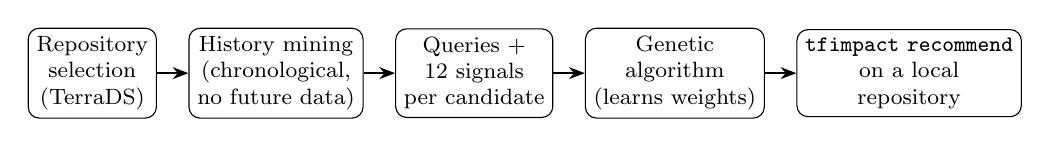
\begin{tikzpicture}[
  box/.style={draw, rounded corners, align=center, font=\footnotesize, minimum height=9mm,
              inner sep=3pt},
  arr/.style={-{Stealth[length=2mm]}, thick},
  node distance=4mm]
\node[box] (sel) {Repository\\selection\\(TerraDS)};
\node[box, right=of sel] (mine) {History mining\\(chronological,\\no future data)};
\node[box, right=of mine] (feat) {Queries +\\12 signals\\per candidate};
\node[box, right=of feat] (ga) {Genetic\\algorithm\\(learns weights)};
\node[box, right=of ga] (rec) {\tool{} \texttt{recommend}\\on a local\\repository};
\draw[arr] (sel) -- (mine);
\draw[arr] (mine) -- (feat);
\draw[arr] (feat) -- (ga);
\draw[arr] (ga) -- (rec);
\end{tikzpicture}
\caption{\small Overview: from repository selection to the recommendation tool.}
\label{fig:pipeline}
\end{figure}

\subsection{Signals}
Table~\ref{tab:features} lists the signals, all scaled to $[0, 1]$, in 3 families. The
\textbf{History} family mines \textbf{association rules} from the repository's own earlier commits, as
ROSE~\cite{zimmermann2004rose} does, at 3 granularities: between blocks, between files, and
between block types; the type-level rule (``adding a bucket goes with adding a bucket policy'') is
the only history signal available for new blocks.

The \textbf{Graph} family uses the reference graph of the repository before the commit, including the links a module call creates to another directory; shared neighbors are weighted with the Adamic--Adar index~\cite{adamic2003friends}, so a shared rare neighbor counts more than a shared hub such as a common tags variable. The propagation rule is mined: it learns from earlier commits how often a direct neighbor changes, separately for added, modified and removed seeds and for each edge direction, because a removed block breaks its referencers far more often than an edited one.

The \textbf{Text} family compares names and the contents of the blocks (TF-IDF over the tokens of their bodies), which links copies of a configuration that no reference connects. Every signal is computed per repository and only from data available before the commit (Section~\ref{sec:problem}).

\begin{table}[ht]
\begin{tabular}{@{}l>{\raggedright\arraybackslash}p{10.2cm}@{}}
\toprule
Signal & Definition \\
\midrule
\multicolumn{2}{@{}l}{\emph{History} (earlier commits of the repository)} \\
\textbf{co-change confidence} & share of past commits changing $s$ that also changed $c$ \\
\textbf{co-change count}      & number of past commits changing both (log-scaled) \\
\textbf{co-change recency}    & co-changes weighted by how recent they are \\
\textbf{recent changes}      & how often $c$ changed in the last 200 commits \\
\textbf{file confidence}      & the same rule between the files of $s$ and $c$ \\
\textbf{type rule}            & rule between block types, e.g.\ modified \texttt{variable} $\Rightarrow$ changed \texttt{module}; for types to add, $\Rightarrow$ added type \\
\midrule
\multicolumn{2}{@{}l}{\emph{Graph} (references before the commit)} \\
proximity            & $1/(1+d)$ for reference distance $d \le 4$, else 0 \\
\textbf{shared neighbors}    & Adamic--Adar score of common neighbors \\
\textbf{degree}              & number of references of $c$ \\
\textbf{propagation rule}     & learned rate at which direct neighbors change, per seed action and edge direction \\
\midrule
\multicolumn{2}{@{}l}{\emph{Text}} \\
\textbf{name similarity}      & overlap of name tokens; for types to add, seed name vs.\ type name \\
\textbf{content similarity}   & TF-IDF cosine of the seed's new body and the candidate's body \\
\bottomrule
\end{tabular}
\centering
\footnotesize
\caption{The 12 engineered features relating a seed $s$ to a candidate $c$.}
\label{tab:features}
\end{table}

\subsection{Scoring Model}
A candidate with signal vector $\mathbf{x}$ receives the score
\[
  \mathit{score}(\mathbf{x}) = \mathbf{w}^\top \mathbf{x} + b \cdot [\text{$c$ is a type to add}],
  \qquad w_i \ge 0,\ \textstyle\sum_i w_i = 1,\ b \in [-1, 1].
\]
Each weight reads as the share of trust in one signal. The offset $b$ is needed because a type to
add has only two non-zero signals (type rule and name similarity), so without it such candidates
would always rank below existing blocks, or above them if those two weights grew. Weights are
non-negative because every signal was designed so that a higher value means a stronger relation;
a check that allows negative weights confirms this (Section~\ref{sec:results}).

\subsection{Genetic Algorithm}
The 13 parameters ($\mathbf{w}$ and $b$) are learned by a Genetic Algorithm implemented from
scratch. A chromosome holds the 13 real-valued genes; after every variation step the
weights are clipped at zero and normalized to sum 1, and the offset is clipped to $[-1, 1]$. The
fitness is the \emph{MRR} obtained with the chromosome's weights on a fixed sample of 5,000 training
queries, with the same number of queries from every training repository so that large
repositories do not dominate.

Evaluating on a sample instead of all ${\sim}44$k training queries is
a form of fitness approximation~\cite{jin2005fitness}: a check on one fold gave the same test MRR
at a ninth of the cost. The fitness of the whole population is computed with one matrix product.
Parents are chosen by tournament selection (size 3) and recombined with BLX-$\alpha$ crossover
($\alpha = 0.5$)~\cite{eshelman1993blx}; Gaussian mutation uses a step size that shrinks from 0.2
to 0.02 over the run, and the two best individuals survive unchanged (elitism).

The remaining settings were not assumed but tuned on training data only. A convergence check with
a generous budget (200 generations) showed that validation MRR barely improves after 60 generations
of 60 individuals (0.735 vs.\ 0.738), which fixed the budget at about 3,600 fitness evaluations. Within each \textbf{cross-validation fold}, a \textbf{grid search} over population/generations at that budget, mutation rate and crossover rate (27 configurations, 3 runs each) trained on 75\% of the training repositories and selected the
configuration with the best MRR on the other 25\%. The final model, trained on all 53 repositories,
uses a population of 30, 120 generations, a mutation rate of 0.1 and a crossover rate of 0.8.

\subsection{The \tool{} Tool}
The command \texttt{tfimpact recommend --repo PATH --diff} applies the final model to a local
Terraform repository. It mines the repository's history with the same pipeline, takes the blocks
changed in the working tree as seeds (or a single block given with \texttt{--block}), and prints
the top blocks to modify and block types to add; \texttt{--explain} shows the signals behind each
suggestion. It needs only Git and the 13 learned numbers, and runs in a few seconds on a
repository with a few hundred commits.

% \section{Evaluation Setup}
\label{sec:evaluation}

\paragraph{Protocol.} We use grouped 5-fold cross-validation over repositories: the 53 core
repositories are split into five folds of similar query count, and every fold is tested with
weights learned on the other four, so each repository is scored by a model that never saw it. Only
the 13 weights cross repositories; all signals are always computed within a repository. The grid
search runs inside each fold on training repositories only, and the genetic algorithm is run with
10 seeds per fold. The 8 held-out repositories are never trained on and are scored with every
fold's model.

\paragraph{Metrics.} The primary metric is the \emph{mean reciprocal rank} (MRR), the inverse rank of
the first true answer, which is also the fitness. We also report \emph{mean average precision} (MAP),
which rewards ranking \emph{all} true answers high, and Hit@$k$, the share of queries with a true
answer in the top $k$ (the success rate used by GA-IaCRec~\cite{bessghaier2026iacrec}). Metrics
are averaged per repository and then over repositories, so every repository counts equally. They
are reported for two target sets: \textbf{all targets} (existing blocks and types to add) and the
stricter \textbf{existing blocks only}.

\paragraph{Comparisons.} For RQ1, the GA is compared with a \emph{random ranking} (the
floor for feasibility) and with \emph{random search}, which draws as many random weight vectors as
the genetic algorithm evaluates and keeps the best one; two further checks retrain it with the
labels shuffled within each query, which must destroy what it learns, and with negative weights
allowed. For RQ2, it is compared with ROSE~\cite{zimmermann2004rose}, run with its original
settings (rules with support $\ge 1$ and confidence $\ge 0.1$, top 10, the type rule for new
blocks), and with \emph{equal weights}, the average of the same twelve signals, i.e.\ the
unlearned combination that GA-IaCRec uses for its two heuristics.

\paragraph{Statistics.} Following the guidelines of Arcuri and Briand for randomized
algorithms~\cite{arcuri2011stats}, methods are compared on per-repository values ($n = 53$) with
the Wilcoxon signed-rank test, Holm's correction for multiple comparisons~\cite{holm1979}, and the
Vargha--Delaney $\hat{A}_{12}$ effect size~\cite{vargha2000a12}, read as negligible, small, medium
or large at 0.56, 0.64 and 0.71. We also report bootstrap 95\% confidence intervals of the mean.

% \section{Results}
\label{sec:results}

\subsection{RQ1: Feasibility and Reliability of the Genetic Algorithm}
\label{sec:rq1}

Table~\ref{tab:rq1} collects the evidence. \emph{Block-level prediction is feasible}: with the
learned weights, the first true answer is on average close to the top of the list (\textbf{MRR 0.746}),
and 84.6\% of the queries have a true answer among the first five suggestions, against an MRR of
0.118 for a random ranking. Since only 81\% of the true answers are among the candidates at all,
there is little room left at the top.

\begin{table}[ht]
\setlength{\tabcolsep}{4pt}
\begin{tabular}{@{}lcccc@{}}
\toprule
Learner & All targets & 95\% CI & Existing blocks & SD over runs \\
\midrule
\textbf{Genetic algorithm}      & \textbf{0.746} $\pm$ 0.076 & [0.727, 0.766] & \textbf{0.649} $\pm$ 0.110 & 0.0008 \\
Random search, same budget      & 0.733 $\pm$ 0.079 & [0.713, 0.754] & 0.644 $\pm$ 0.110 & 0.0031 \\
GA, negative weights allowed    & 0.742 $\pm$ 0.079 & [0.721, 0.763] & 0.641 $\pm$ 0.117 & -- \\
GA, labels shuffled in training & 0.428 $\pm$ 0.181 & [0.380, 0.476] & 0.461 $\pm$ 0.172 & -- \\
Random ranking                  & 0.118 $\pm$ 0.037 & [0.108, 0.128] & 0.116 $\pm$ 0.037 & -- \\
\bottomrule
\end{tabular}
\centering
\small
\caption{RQ1: GA evaluation (53 repositories; MRR as mean $\pm$ SD over
repositories, 95\% bootstrap CI of the mean for all targets; last column: SD of the mean over the
10 runs per fold).}
\label{tab:rq1}
\end{table}

\emph{The GA learns from the labels.} Retrained on labels shuffled within each query, it drops to
0.428, below even the unlearned equal weights (0.563), so its result comes from the relation
between signals and true answers, not from an artefact of the data. \emph{It converges reliably.}
Validation MRR rises quickly and is almost flat after 60 generations
(Figure~\ref{fig:convergence}); the mean MRR varies by only 0.0008 across the ten runs per fold, and the 27 grid
configurations by at most 0.010, so the result depends neither on the seed nor on the settings.
Allowing negative weights changes nothing (0.742) and no signal receives a negative mean weight,
which confirms the non-negativity constraint.

\emph{Against random search} with the same number of evaluations, the GA is better on 50 of 53
repositories ($p < 10^{-8}$) and four times more stable across runs, but the margin is small
(+0.013 MRR, negligible $\hat{A}_{12} = 0.56$). With only 13 continuous parameters, random sampling
already finds good weights: the GA is a useful optimizer here rather than a decisive one. The
learned weights (Figure~\ref{fig:weights}) concentrate on 3 signals: the propagation rule
(0.31), the type rule (0.20) and content similarity (0.18), with an offset of 0.21 for types to add.

\begin{figure}[ht]
\centering
\begin{subfigure}[t]{0.49\textwidth}
  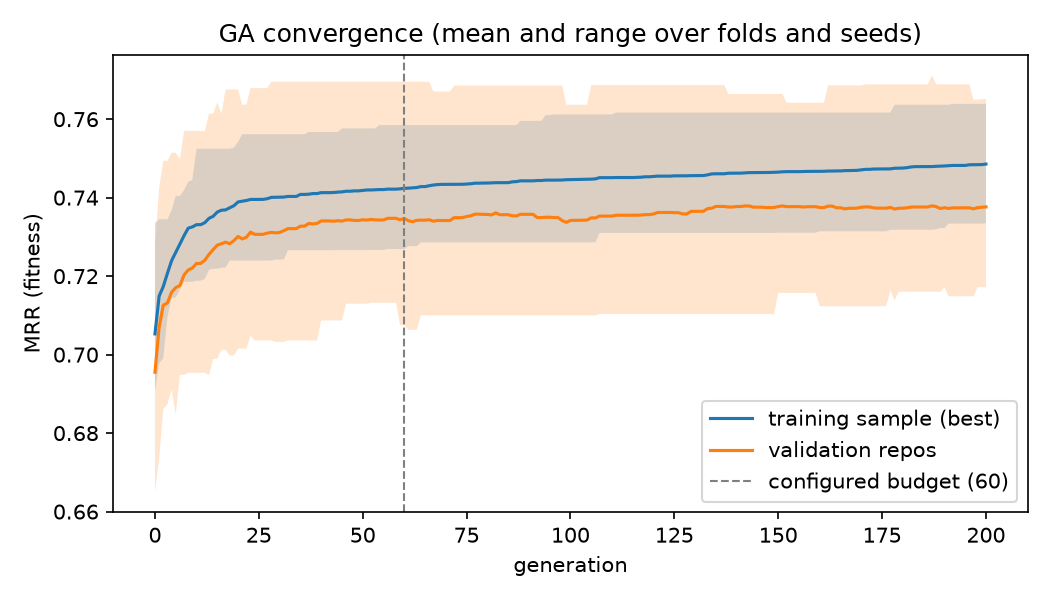
\includegraphics[width=\linewidth]{fig/convergence.png}
  \caption{Convergence: best training fitness and validation MRR per generation.}
  \label{fig:convergence}
\end{subfigure}\hfill
\begin{subfigure}[t]{0.49\textwidth}
  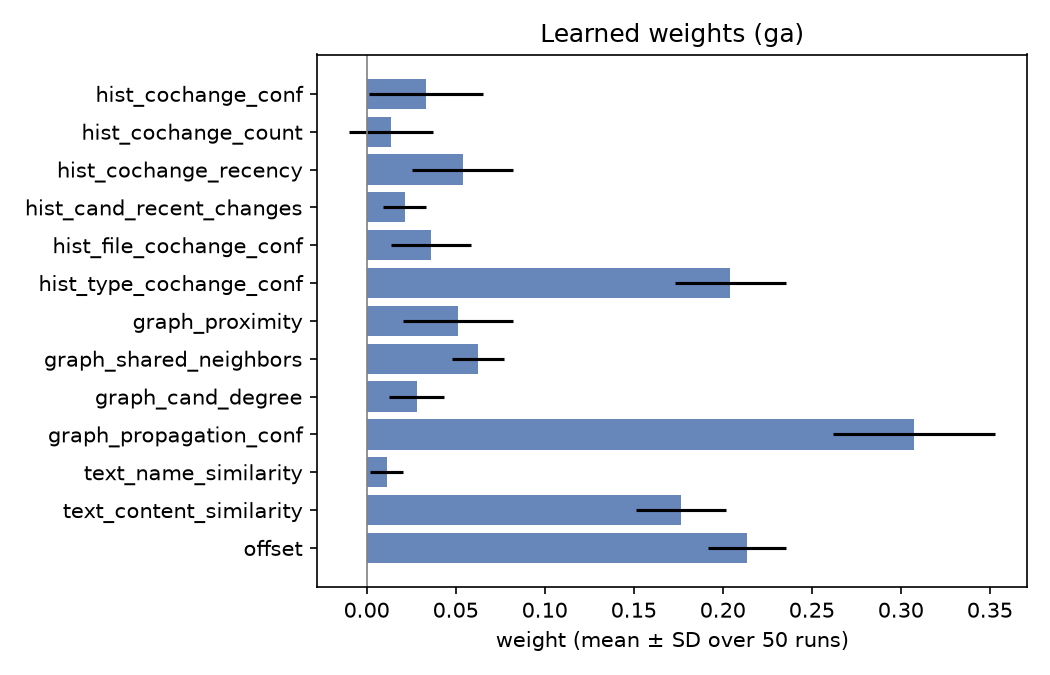
\includegraphics[width=\linewidth]{fig/learned_weights_ga.png}
  \caption{Learned weights (mean $\pm$ SD over 50 runs).}
  \label{fig:weights}
\end{subfigure}
\caption{RQ1: behavior of the Genetic Algorithm.}
\end{figure}

\subsection{RQ2: Learned Ranking vs.\ Prior Work and Equal Weights}
\label{sec:rq2}

Table~\ref{tab:rq2} compares the learned ranking with ROSE and with equal weights. On all targets
the GA is better than both on almost every repository, with large effect sizes: +0.27 MRR over ROSE
(53 of 53 repositories) and +0.18 over equal weights (51 of 53). It is also more consistent across
repositories (SD 0.076 vs.\ 0.147 for equal weights). On the 8 held-out repositories, never used
for training, it reaches 0.716, against 0.177 for equal weights.

\begin{table}[ht]
\setlength{\tabcolsep}{4pt}
\begin{tabular}{@{}llccccc@{}}
\toprule
Targets & Method & MRR & 95\% CI & MAP & Hit@5 & GA better / worse, $\hat{A}_{12}$ \\
\midrule
\multirow{3}{*}{All}
 & \textbf{GA}   & \textbf{0.746} $\pm$ 0.076 & [0.727, 0.766] & \textbf{0.437} & \textbf{0.846} & -- \\
 & Equal weights & 0.563 $\pm$ 0.147 & [0.526, 0.601] & 0.332 & 0.670 & 51 / 2, 0.87 \\
 & ROSE          & 0.481 $\pm$ 0.152 & [0.443, 0.522] & 0.231 & 0.555 & 53 / 0, 0.93 \\
\midrule
\multirow{3}{*}{Existing}
 & \textbf{GA}   & \textbf{0.649} $\pm$ 0.110 & [0.622, 0.680] & 0.439 & 0.755 & -- \\
 & Equal weights & 0.644 $\pm$ 0.106 & [0.617, 0.673] & \textbf{0.444} & \textbf{0.769} & 32 / 21, 0.52 (n.s.) \\
 & ROSE          & 0.360 $\pm$ 0.164 & [0.318, 0.405] & 0.211 & 0.440 & 53 / 0, 0.91 \\
\bottomrule
\end{tabular}
\centering
\small
\caption{RQ2: comparison with ROSE and equal weights (53 repositories; MRR as mean $\pm$ SD over
repositories with 95\% bootstrap CI). Paired tests on per-repository MRR: repositories where the GA
is better / worse and $\hat{A}_{12}$; all $p < 10^{-8}$ except where marked n.s.}
\label{tab:rq2}
\end{table}

The gain is not uniform (Figure~\ref{fig:seedaction}). It comes from \emph{added} seeds (0.732 vs.\
0.388 for equal weights), where the learned offset places the types to add correctly, and from
\emph{removed} seeds (0.853 vs.\ 0.774), driven by the propagation rule. On \emph{existing blocks}
alone the GA and equal weights are statistically tied (0.649 vs.\ 0.644, $p = 0.19$): equal
weights are already close to the best \emph{linear} combination there. ROSE stays behind everywhere
because most true answers have no earlier co-change with the seed.

\subsection{Ablation Study: Contribution of the Signal Families}
\label{sec:ablation}

To see what each signal family contributes, we retrained the GA on one family at a time (the
design of GA-IaCRec's ablation~\cite{bessghaier2026iacrec}, with learned weights; 3 runs per fold).
Every family alone is clearly worse than the combination, on all 53 repositories
(Table~\ref{tab:ablation}), and each covers a different kind of edit
(Figure~\ref{fig:ablationseed}): history carries added seeds through the type rule, the graph
carries removed seeds through the propagation rule, and text is the strongest single family for
modified seeds and on existing blocks.

\begin{table}[ht]
\setlength{\tabcolsep}{4pt}
\begin{tabular}{@{}lccccc@{}}
\toprule
Signals & All targets & 95\% CI & Existing blocks & RI (all / existing) & $\hat{A}_{12}$ (all) \\
\midrule
\textbf{GA-FULL} & \textbf{0.745} $\pm$ 0.076 & [0.727, 0.766] & \textbf{0.648} $\pm$ 0.112 & -- & -- \\
GA-HIST (6) & 0.660 $\pm$ 0.097 & [0.635, 0.685] & 0.497 $\pm$ 0.142 & +13\% / +31\% & 0.76 \\
GA-TEXT (2)    & 0.488 $\pm$ 0.162 & [0.445, 0.533] & 0.533 $\pm$ 0.145 & +53\% / +22\% & 0.92 \\
GA-GRAPH (4)   & 0.420 $\pm$ 0.112 & [0.392, 0.450] & 0.460 $\pm$ 0.114 & +78\% / +41\% & 0.99 \\
\bottomrule
\end{tabular}
\centering
\small
\caption{Ablation: the GA trained on one signal family (MRR as mean $\pm$ SD over repositories,
95\% bootstrap CI for all targets; RI = relative improvement of the full model over the variant;
full model better on 53 of 53 repositories in all targets, $p < 10^{-8}$).}
\label{tab:ablation}
\end{table}

\begin{figure}[ht]
\centering
\begin{subfigure}[t]{0.49\textwidth}
  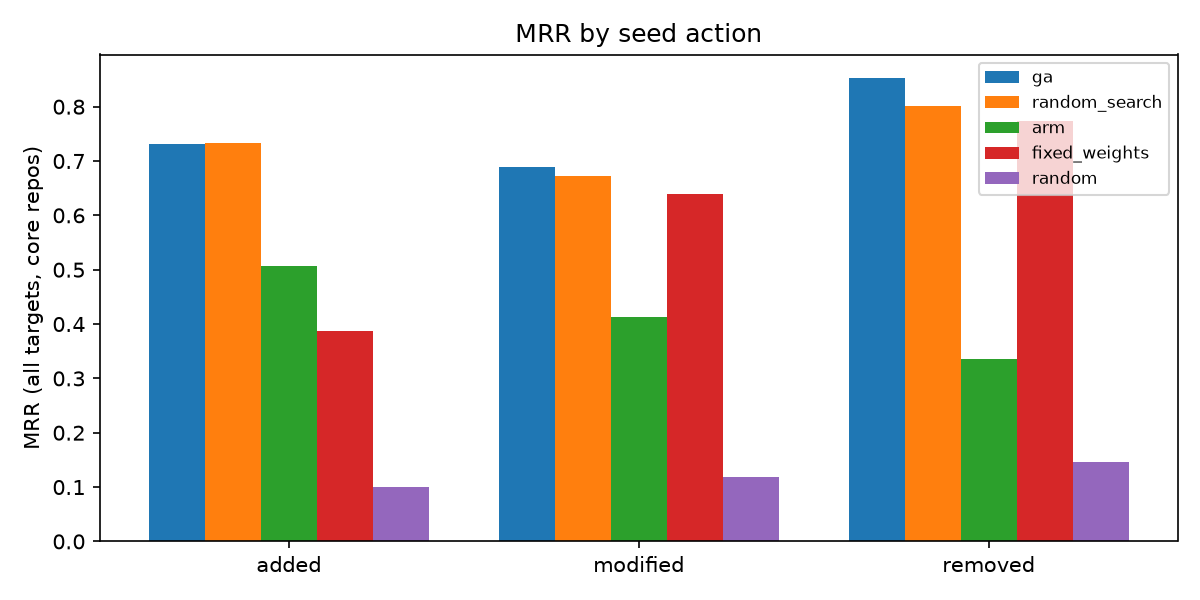
\includegraphics[width=\linewidth]{fig/mrr_by_seed_action.png}
  \caption{RQ2: GA, random search, ROSE (\texttt{arm}), equal weights (\texttt{fixed\_weights})
  and random ranking.}
  \label{fig:seedaction}
\end{subfigure}\hfill
\begin{subfigure}[t]{0.49\textwidth}
  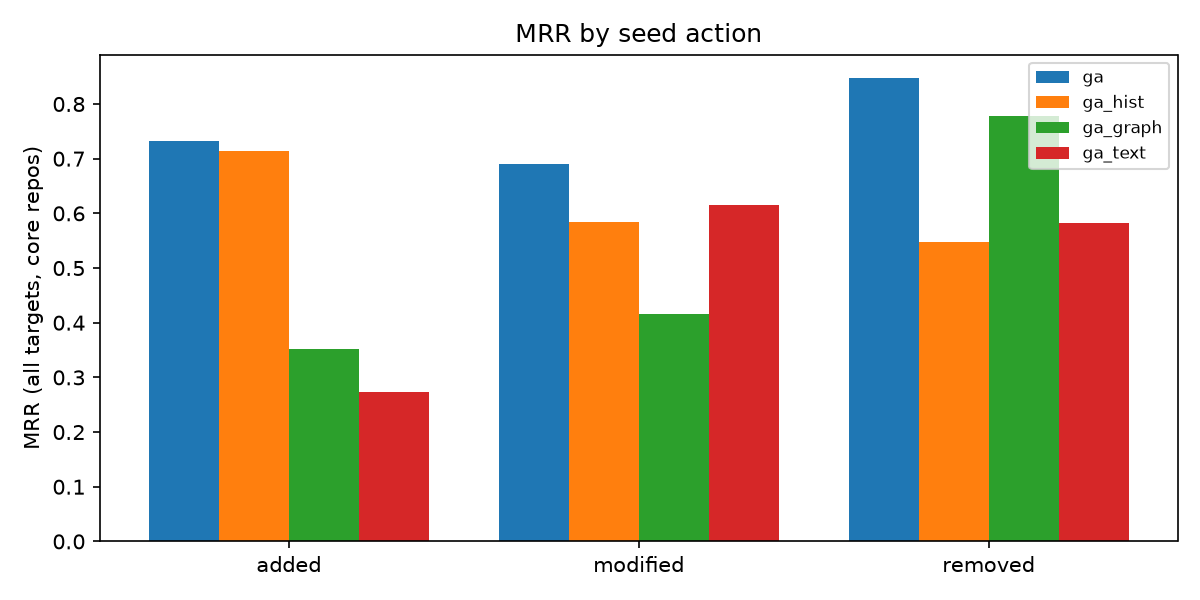
\includegraphics[width=\linewidth]{fig/ablation_seed_action.png}
  \caption{Ablation: full model vs.\ one family at a time.}
  \label{fig:ablationseed}
\end{subfigure}
\caption{MRR (all targets) by the action of the seed block.}
\end{figure}

Finally, the amount of training data matters little. Trained on 10, 25, 50 or 75\% of each fold's
training repositories, the GA reaches a test MRR of 0.734, 0.743, 0.747 and 0.744, against 0.745
with all of them: the curve is flat from about ten repositories, and training and test MRR stay
within 0.01 of each other at every size. More data would therefore not improve the model; its
linear form is the limit, which we return to in Section~\ref{sec:discussion}.

% \section{Discussion}
\label{sec:discussion}

\paragraph{The linear score is the limit.} Learning pays off where one weight vector must place 2
kinds of candidates or reward a rare but strong signal (added and removed seeds), but on existing
blocks the learned weights only tie equal weights, and more training data does not help. What is
missing is not data but interactions: a signal's value depends on context (the propagation rule
matters for removed seeds, content similarity for copies), which a single linear score cannot
express.

\paragraph{Learning matters more than the optimizer.} Random search with the same budget comes within 0.013 MRR
of the GA, and the GA's settings barely matter. The contribution lies more in \emph{learning} the
combination from mined labels than in the choice of optimizer; a harder search space, such as
evolving the scoring formula itself, would put the GA to a stronger test.

\paragraph{Scope and limitations.} \emph{Labels are co-changes, not necessary changes}: a commit may bundle
unrelated edits or leave a required one for later, which makes the results pessimistic rather than
optimistic. The repositories use AWS only, and thresholds and signals were designed while looking at
the same repositories that were later evaluated (the learned weights never saw their test
repositories, but our design choices did). Finally, the history is limited to the last 2,000
commits, the condition under which the model was evaluated.

% \section{Conclusions and Future Work}
\label{sec:conclusions}

This report addressed change impact analysis for Terraform: given an edited block, which other
blocks will change with it, and which blocks will be added? We mined a dataset from 53 open-source
repositories and learned, with a self-implemented Genetic Algorithm, how to combine twelve signals
from the repository's history, reference graph and text. \textbf{RQ1}: the Genetic Algorithm is a
feasible and reliable learner for this task: it learns from the labels, converges within about 60
generations and gives almost identical results across runs and settings, although random search
with the same budget comes close. \textbf{RQ2}: the learned ranking clearly outperforms
history-based rule mining (ROSE) and equal weights, mainly by placing new block types and by
following references from removed blocks, and the three signal families are complementary. The
\tool{} tool makes the learned model usable on any local Terraform repository.

Future work follows from the limits above. Non-linear rankers, such as gradient-boosted ranking
models or Genetic Programming (GP) that evolves the scoring formula, could capture the interactions a
linear score misses and give the evolutionary search a harder problem; a simpler step is separate
weights per seed action. An independent sample of new repositories would test the design choices
as well as the weights, and other cloud providers and IaC languages would test generality. For
everyday use, caching the mined history would make repeated recommendations instant.


\bibliographystyle{alpha}
\bibliography{biblio}

\end{document}
